%%=============================================================================
%% Implementatie
%%=============================================================================

\chapter{Ontwerp en implementatie van het AI-gestuurde dashboard}
\label{ch:implementatie}

\section{Architectuur van het systeem}
% hoog niveau: frontend, backend, database, AI-laag, integratie met GitHub/n8n/Mastra

\section{Implementatie van de Mastra-agent}
\label{sec:mastra-implementatie}

Voor de eerste AI-integratie wordt gebruikgemaakt van Mastra, een TypeScript framework om AI-agents, tools en workflows te definiëren en te orchestreren. In de proof-of-concept wordt een \texttt{dependencyAgent} opgezet die specifiek is afgestemd op het analyseren van npm-dependency-updates. Deze agent combineert een taalmodel (bijvoorbeeld Google's \texttt{gemini-2.5-flash} of OpenAI's \texttt{gpt-4o-mini}) met twee eigen tools: \texttt{fetchNpmInfoTool} en \texttt{webChangelogSearchTool}.

De agent volgt een gestructureerde research-strategie: eerst haalt de \texttt{fetchNpmInfoTool} metadata en releasenotes op uit npm en GitHub; als die incompleet zijn, volgt de \texttt{webChangelogSearchTool} met een gerichte webzoekopdracht naar changelogs. Het resultaat wordt gecombineerd en volgens een strikt JSON-formaat geformatteerd, zodat ontwikkelaars direct actionable inzichten krijgen over features, breaking changes, security fixes en migratiestappen. Listing~\ref{lst:mastra-agent-config} toont de definitie van de agent.

\begin{listing}[H]
\begin{minted}{typescript}
import { Agent } from "@mastra/core/agent";
import { google } from "@ai-sdk/google";
import { fetchNpmInfoTool } from "../tools/npm-tool";
import { webChangelogSearchTool } from "../tools/web-changelog-search-tool";

const MODEL = google("gemini-2.5-flash");

export const dependencyAgent = new Agent({
  id: "DependencyAnalyzer",
  name: "Dependency Analyzer",
  instructions: `
    You are a dependency update analyst for software developers.
    Your goal is to give developers CONCRETE, SPECIFIC information about package 
    updates so they do NOT have to read the full changelog themselves.

    ## Research Strategy (follow IN ORDER)

    ### Step 1 — fetch-npm-info
    Always start by calling the fetch-npm-info tool with:
    - packageName, fromVersion, toVersion

    ### Step 2 — web-changelog-search  
    Call web-changelog-search when npm tool returns "No release notes found".

    ## Output Format
    ## [package-name] v[from] → v[to] ([major/minor/patch] update)

    > Source: [tool source or URL]

    ### New Features     ### Breaking Changes
    ### Security Fixes   ### Deprecated
    ### Migration Steps  ### Safe to update?
  `,
  model: MODEL,
  tools: {
    fetchNpmInfoTool,
    webChangelogSearchTool,
  },
});
\end{minted}
\caption{Mastra \texttt{dependencyAgent}-configuratie met tools en research-strategie}
\label{lst:mastra-agent-config}
\end{listing}

De \texttt{fetchNpmInfoTool} (Listing~\ref{lst:npm-tool}) is de primaire tool voor het ophalen van npm-metadata en GitHub-release notes. De tool zoekt eerst naar een exacte release-tag (bijvoorbeeld \texttt{v1.2.3}), valt terug op de laatste vijf releases als die niet bestaat, en probeert vervolgens CHANGELOG-bestanden (\texttt{CHANGELOG.md}, \texttt{HISTORY.md}, …) uit de repository te lezen. Dankzij fallback-logica en robuuste foutafhandeling levert de tool altijd een gestructureerd resultaat, zelfs als er geen officiële release notes zijn.

\begin{listing}[H]
\begin{minted}[linenos=false]{typescript}
export const fetchNpmInfoTool = createTool({
  id: "fetch-npm-info",
  inputSchema: z.object({
    packageName: z.string(),
    fromVersion: z.string(),
    toVersion: z.string(),
  }),
  execute: async ({ packageName, fromVersion, toVersion }) => {
    // 1. npm registry metadata
    const npmData = await fetch(`https://registry.npmjs.org/${packageName}`).then(r => r.json());

    // 2. GitHub releases (exact tag, dan recentste, dan CHANGELOG.md)
    const repoMatch = npmData.repository?.url?.match(/github\.com[/:]([\w.-]+\/[\w.-]+)/);
    if (repoMatch) {
      const [tagRes] = await Promise.allSettled([
        // Try exact tag variants
        ...["v${toVersion}", toVersion].map(tag => 
          fetch(`https://api.github.com/repos/${repoMatch[1]}/releases/tags/${tag}`)
            .then(r => r.json())
        )
      ]);
      // ... fallback naar CHANGELOG parsing
    }

    return {
      description: npmData.description || "",
      homepage: npmData.homepage || "",
      repository: npmData.repository?.url || "",
      releaseNotes: releaseNotes || "No release notes found on GitHub.",
      changelogUrl,
      source,
    };
  },
});
\end{minted}
\caption{\texttt{fetchNpmInfoTool}: npm-metadata en GitHub release notes met CHANGELOG fallback}
\label{lst:npm-tool}
\end{listing}

Als de npm-tool geent nuttige release notes vindt, volgt de \texttt{webChangelogSearchTool} (Listing~\ref{lst:web-search-tool}). Deze tool voert een gerichte webzoekopdracht uit naar changelogs via Tavily, Brave Search of DuckDuckGo, met domeinpriorisering voor officiële package-sites (bijvoorbeeld \texttt{nextjs.org}, \texttt{angular.dev}). De tool prioriteert resultaten van officiële documentatie boven aggregators en levert een lijst van relevante titels, URL's en snippets.

\begin{listing}[H]
\begin{minted}[linenos=false]{typescript}
export const webChangelogSearchTool = createTool({
  id: "web-changelog-search",
  inputSchema: z.object({
    packageName: z.string(),
    fromVersion: z.string(),
    toVersion: z.string(),
  }),
  execute: async ({ packageName, fromVersion, toVersion }) => {
    const query = buildQuery(packageName, fromVersion, toVersion);
    
    if (process.env.TAVILY_API_KEY) {
      return await searchWithTavily(query, packageName, toVersion);
    }
    return await searchWithDuckDuckGo(query); // fallback
  },
});
\end{minted}
\caption{\texttt{webChangelogSearchTool}: webzoekopdracht naar changelogs en migratieguides}
\label{lst:web-search-tool}
\end{listing}

De Mastra-agent wordt vanuit de Next.js-backend aangeroepen via een API-route die de dependency-gegevens doorstuurt en de gestructureerde output opslaat in Supabase. Door de combinatie van deze twee tools en de expliciete instructies levert de agent betrouwbare, actionable samenvattingen die ontwikkelaars tijd besparen bij het beoordelen van updates.

\section{Implementatie van de n8n-workflow}
\label{sec:n8n-implementatie}

Als tweede AI-integratie wordt een n8n-workflow opgezet die dezelfde kernfunctie vervult als de Mastra-agent, maar dan in een low-code, visueel georkestreerde omgeving. De workflow ontvangt een HTTP-aanvraag vanuit de webapplicatie, verrijkt de aangeleverde dependency-informatie met data uit npm, Github en een webzoekdienst (Tavily)\footnote{Tavily is een API en infrastructuurlaag die AI-agents en LLM-toepassingen real-time toegang geeft tot webzoekopdrachten, webextractie en crawling.\url{https://www.tavily.com/}}, en laat vervolgens een AI-model (Gemini 2.5 flash) een samenvatting genereren van de relevante wijzigingen. Het resultaat wordt teruggestuurd naar de applicatie via de webhook-respons en opgeslagen in de databank.

De workflow bestaat uit een keten van acht nodes (Figuur~\ref{fig:n8n-workflow}):

\begin{itemize}
    \item \textbf{Node 1: Webhook.} Deze node fungeert als ingangspunt voor de workflow en wordt getriggerd zodra de Next.js-backend een HTTP-aanvraag naar de n8n-URL stuurt. De node is geconfigureerd om te antwoorden via een aparte \emph{Respond to Webhook}-node, zodat alle tussenliggende stappen eerst afgewerkt worden.
    \item \textbf{Node 2: npm-metadata (Code).} In deze code-node wordt de JSON-body van de inkomende request uitgelezen (\texttt{packageName}, \texttt{fromVersion}, \texttt{toVersion}) en wordt via \texttt{this.helpers.httpRequest } een call gedaan naar \\ \texttt{ https://registry.npmjs.org/\{packageName\}}. De node reconstrueert de repository-URL uit de npm-metadata en geeft een nieuwe JSON-object door met omschrijving, homepage en repository-informatie.
    \item \textbf{Node 3: Github-node (Code).} Deze node ontvangt de verrijkte npm-data, extraheert \texttt{owner/repo} uit de repository-URL en probeert via de Github API eerst release notes op te halen voor de specifieke tag (\texttt{v\{toVersion\}} of \texttt{toVersion}). Als die niet gevonden wordt, heelt de node de laatste releases op en concateneert de body-teksten tot een \texttt{releaseNotes}-veld. Als er ook geen releases zijn, wordt er nog geprobeerd een \texttt{CHANGELOG.md}, \texttt{CHANGES.md} of \texttt{HISTORY.md} rechtstreeks uit de repository te lezen. De node voegt \texttt{releaseNotes}, \texttt{changelogUrl} en \texttt{source} toe aan de JSON.
    \item \textbf{Node 4: HTTP Request (Tavily).} Via een HTTP-request-node wordt de Tavily API aangeroeperen om webresultaten op te halen die extra context kunnen geven over de dependency of de update (bijvoorbeeld blogposts of documentatie rond de nieuwe versie).
    \item \textbf{Node 5: Merge-node (Code).} Deze node voegt de Github-data en Tavily-resultaten samen. De webresultaten worden omgezet naar een tekstveld \texttt{webSnippets} (titel, URL en inhoud per resultaat), dat samen met de eerder verzamelde metadata en release notes wordt doorgegeven aan de AI-node.
    \item \textbf{Node 6: AI-agent (Gemini).} Een AI-node, geconfigureerd met het model \texttt{gemini-2.5-flash}, ontvangt \texttt{releaseNotes}, \texttt{webSnippets} en versie-informatie als input. Met behulp van een system prompt en user prompt genereert het model een gestructureerde samenvatting van de update (bijvoorbeeld features, breaking changes, security-aspecten en migratieadvies).
    \item \textbf{Node 7: Code-node (post-processing).} Deze node extraheert de relevante output uit de AI-respons (bijvoorbeeld \texttt{output} of \texttt{summary}) en zet die om naar een eenvoudige JSON-object met één veld \texttt{summary}, zodat de webhook-respons helder en compact blijft.
    \item \textbf{Node 8: Respond to Webhook.} De laatste node stuurt de \texttt{summary} terug als HTTP-respons naar de oorspronkelijke aanroeper. Aan de kant van de webapplicatie kan deze samenvatting vervolgens rechtstreeks worden opgeslagen in de databank.
\end{itemize}

De Next.js-backend roept de n8n-workflow aan via een dedicated route (vereenvoudigd weergegeven in Listing~\ref{lst:n8n-route}). Deze route valideert eerst de gebruiker met Supabase, leest de dependencygegevens uit de inkomende request (\texttt{dependencyId}, \texttt{name}, \texttt{currentVersion}, \texttt{latestVersion}) en stuurt die als JSON-payload door naar de n8n-webhook. De samenvatting die n8n terugstuurt wordt daarna opgeslagen in het veld \texttt{ai\_summary} van de desbetreffende dependency.

\begin{listing}[H]
\begin{minted}{ts}
export async function POST(request: Request) {
  const supabase = await createClient();
  const { data: { user } } = await supabase.auth.getUser();
  if (!user) {
    return NextResponse.json({ error: "Unauthorized" }, { status: 401 });
  }

  const { dependencyId, name, currentVersion, latestVersion } =
    await request.json();

  const n8nRes = await fetch(
    process.env.N8N_WEBHOOK_URL ?? "http://localhost:5678/webhook-test/analyze-dependency",
    {
      method: "POST",
      headers: { "Content-Type": "application/json" },
      body: JSON.stringify({
        packageName: name,
        fromVersion: currentVersion,
        toVersion: latestVersion,
      }),
    }
  );

  const n8nData = await n8nRes.json();
  const summary = n8nData.summary;

  await supabase
    .from("dependencies")
    .update({ ai_summary: summary })
    .eq("id", dependencyId);

  return NextResponse.json({ summary });
}
\end{minted}
\caption[Aanroep van de n8n-workflow]{Next.js-route die de n8n-workflow aanroept en de samenvatting opslaat}
\label{lst:n8n-route}
\end{listing}

Figuur~\ref{fig:n8n-workflow} toont de volledige n8n-workflow zoals geïmplementeerd in deze bachelorproef, met de opeenvolgende nodes van inkomnde webhook tot AI-gegenereerde samenvatting.

\begin{figure}[H]
  \centering
  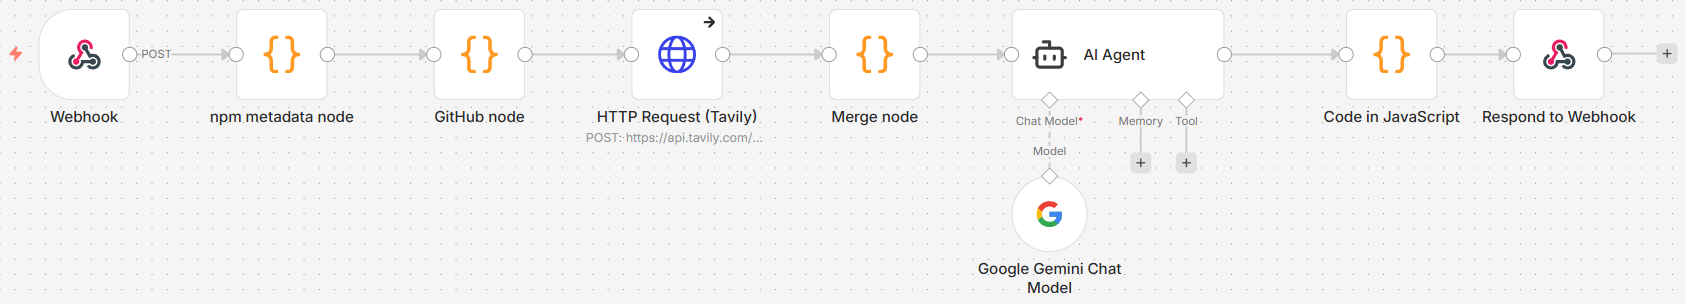
\includegraphics[width=\textwidth,keepaspectratio]{img/n8n-workflow.png}
  \caption[AI-workflow in n8n]{Overzicht van de n8n-workflow die metadata, release notes, webcontext en AI-samenvatting combineert}
  \label{fig:n8n-workflow}
\end{figure}

\section{Integratie met de webapplicatie}
% hoe dashboard de AI-resultaten ophaalt, toont, beslisregels, enz.
